\documentclass[../TDO3.tex]{subfiles}%

\begin{document}
\section[s]"3"{Étude d'un rétroprojecteur}
\enonce{%
	\noindent
	\begin{minipage}[c]{.58\linewidth}
		Un rétroprojecteur est un ensemble lentille-miroir, avec un miroir plan incliné
		à \ang{45;;} par rapport à la lentille. L'ensemble lentille-miroir est réglable
		en hauteur ($h$). On étudie un rétroprojecteur dont la lentille a une vergence
		de $\SI{2.0}{\delta}$, avec une distance lentille-miroir $d = \SI{10}{cm}$.
		\smallbreak
		On désire projeter un objet transparent AB sur un écran placé à $D =
			\SI{3.0}{m}$ de l'axe optique de la lentille.
	\end{minipage}
	\hfill
	\begin{minipage}[c]{.4\linewidth}
		~
		\begin{center}
			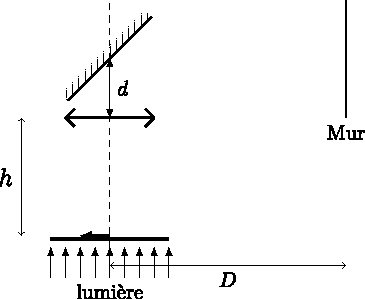
\includegraphics[width=\linewidth]{retroproj}
			\label{fig:retroproj}
		\end{center}
	\end{minipage}
}%

\QR{%
	Déterminer la distance $h$ permettant d'obtenir une image nette sur
	l'écran.
}{%
	On a $\AB \opto{\Lc}{\Or} \ABb \opto{M}{\rm H} \ABp$, avec H le point
	d'intersection entre le miroir plan et l'axe optique de la lentille.
	L'image finale A' donnée par le miroir plan est telle que
	\[
		\boxed{\obar{\rm HA'} = \obar{\rm HA_1} = D}
	\]
	On a donc pour la lentille
	\begin{empheq}[box=\fbox]{align*}
		\obar{\rm OA_1} &= \obar{\rm OH} + \obar{\rm HA_1}
		\\\Lra
		\obar{\rm OA_1} &= d+D
	\end{empheq}
	On utilise la relation de conjugaison des lentilles minces en nommant
	$V$ la vergence de la lentille~:
	\begin{equation*}
		V = \frac{1}{d+D} - \frac{1}{-h}
		\Lra
		\boxed{h = \frac{d+D}{V(d+D)-1}}
		\qav
		\left\{
		\begin{array}{rcl}
			d & = & \SI{10e-2}{m}    \\
			D & = & \SI{3.0}{m}      \\
			V & = & \SI{2.0}{m^{-1}}
		\end{array}
		\right.
	\end{equation*}
	Et l'application numérique donne
	\begin{equation*}
		\xul{h = \SI{60}{cm}}
	\end{equation*}
}%

\QR{%
	Calculer le grandissement.
}{%
	Le miroir plan a un grandissement de 1, donc le grandissement du
	système est celui de la lentille~: on a $\gamma = \DS
		\frac{\ABb}{\AB} = \frac{\obar{\rm OA_1}}{\OA}$, soit
    \begin{align*}
          \gamma &= \frac{d+D}{-h}
          \\\AN
          \makebox[0pt][l]{$\xul{\phantom{\gamma = \num{-5.2}}}$}
          \gamma &= \num{-5.2}
    \end{align*}
}%

\end{document}
